%% ==========================================================================
%% cover/cover.tex : the front cover of JitJet, drawn with TikZ.
%%
%% Compile on its own:   make cover/cover.pdf      (or: cd cover && pdflatex cover)
%% JitJet.tex includes the resulting one-page PDF as the first page of the book.
%%
%% The drawing is the book in one picture. A transverse quarter of CMS sits in
%% the bottom-left corner: beam pipe, tracker layers, ECAL, HCAL, solenoid and
%% the muon system. The b quark (red) is born at the interaction point, showers
%% into gluons (green) and hadrons (gold) inside the jet cone, while pileup
%% tracks (grey, the crowd) come from the same point. The hadrons leave tracks,
%% ECAL and HCAL deposits, a muon that reaches the muon chambers and a neutrino
%% that never arrives. The road along the jet axis leaves the detector and
%% climbs to the top-right corner: reconstruction, PUPPI and clustering, jet
%% energy corrections, b tagging and finally the three-prong top jet. From
%% bottom (b) to top (t). The seven milestones are the seven parts of the book.
%% ==========================================================================
\documentclass[tikz,border=0pt]{standalone}
\usepackage[T1]{fontenc}
\usepackage{lmodern}
\usepackage{tgheros}          % TeX Gyre Heros for the sans-serif title
\usepackage{amssymb}
\usetikzlibrary{calc,arrows.meta,decorations.pathmorphing,shapes.geometric}

%% -------- palette -----------------------------------------------------------
\definecolor{navy}{HTML}{0B1D3A}
\definecolor{navytop}{HTML}{17365F}
\definecolor{gold}{HTML}{F4B942}
\definecolor{bred}{HTML}{FF5A5A}     % b quark  (red in the journey figures)
\definecolor{bblue}{HTML}{6E8EFF}    % bbar     (blue in the journey figures)
\definecolor{fsr}{HTML}{3DD16E}      % FSR gluons (green)
\definecolor{isr}{HTML}{FF9A3C}      % ISR gluon  (orange)
\definecolor{hadroncol}{HTML}{FFC24D}
\definecolor{ecalcol}{HTML}{3FBF77}
\definecolor{hcalcol}{HTML}{E58F2A}
\definecolor{yoke}{HTML}{C24B4B}
\definecolor{steel}{HTML}{9AA7B8}
\definecolor{trackcol}{HTML}{E4ECF7}
\definecolor{pu}{HTML}{8D9AAB}
\definecolor{nucol}{HTML}{5EE7EA}
\definecolor{muoncol}{HTML}{8FB8FF}

%% -------- styles ------------------------------------------------------------
\tikzset{
  ring/.style={draw=steel!70, line width=0.4pt, opacity=0.85},
  tracklayer/.style={draw=bblue!70!white, line width=0.35pt, opacity=0.55},
  bline/.style={draw=bred, line width=1.9pt, line cap=round},
  bbarline/.style={draw=bblue, line width=1.9pt, line cap=round},
  gluon/.style={draw=fsr, line width=0.8pt, decorate,
    decoration={coil, aspect=0.55, segment length=2.4pt, amplitude=1.5pt}},
  isrgluon/.style={gluon, draw=isr},
  quark/.style={draw=hadroncol, line width=0.9pt, line cap=round},
  hadron/.style={circle, fill=hadroncol, draw=navy, line width=0.3pt,
    inner sep=0pt, minimum size=5pt},
  track/.style={draw=trackcol, line width=0.55pt, opacity=0.9},
  photon/.style={draw=hadroncol, line width=0.55pt, dash pattern=on 1.3pt off 1.3pt},
  putrack/.style={draw=pu, line width=0.35pt, opacity=0.4},
  road/.style={draw=white, line width=7pt, opacity=0.09, line cap=round},
  roadline/.style={draw=gold, line width=1pt, dash pattern=on 7pt off 5pt},
  milestone/.style={circle, draw=gold, fill=navy, line width=1.1pt,
    minimum size=13pt, inner sep=0pt, font=\sffamily\bfseries\scriptsize, text=gold},
  mlabel/.style={font=\sffamily\footnotesize, text=white, align=left,
    inner sep=2.5pt, fill=navy, fill opacity=0.75, text opacity=1, rounded corners=1.5pt},
  layerlabel/.style={font=\sffamily\scriptsize, text=white!85!navy, inner sep=1.5pt,
    fill=navy, fill opacity=0.7, text opacity=1, rounded corners=1pt},
}
\newcommand{\sub}[1]{\\{\scriptsize\color{gold!85!white}#1}}

%% radial calorimeter bars: \ecalbar{angle}{height}{colour}, \hcalbar{...}
\newcommand{\ecalbar}[3]{%
  \fill[#3] ({#1-0.9}:5.9) -- ({#1+0.9}:5.9) -- ({#1+0.9}:{5.9+#2}) -- ({#1-0.9}:{5.9+#2}) -- cycle;}
\newcommand{\hcalbar}[3]{%
  \fill[#3] ({#1-1.4}:7.5) -- ({#1+1.4}:7.5) -- ({#1+1.4}:{7.5+#2}) -- ({#1-1.4}:{7.5+#2}) -- cycle;}

\begin{document}
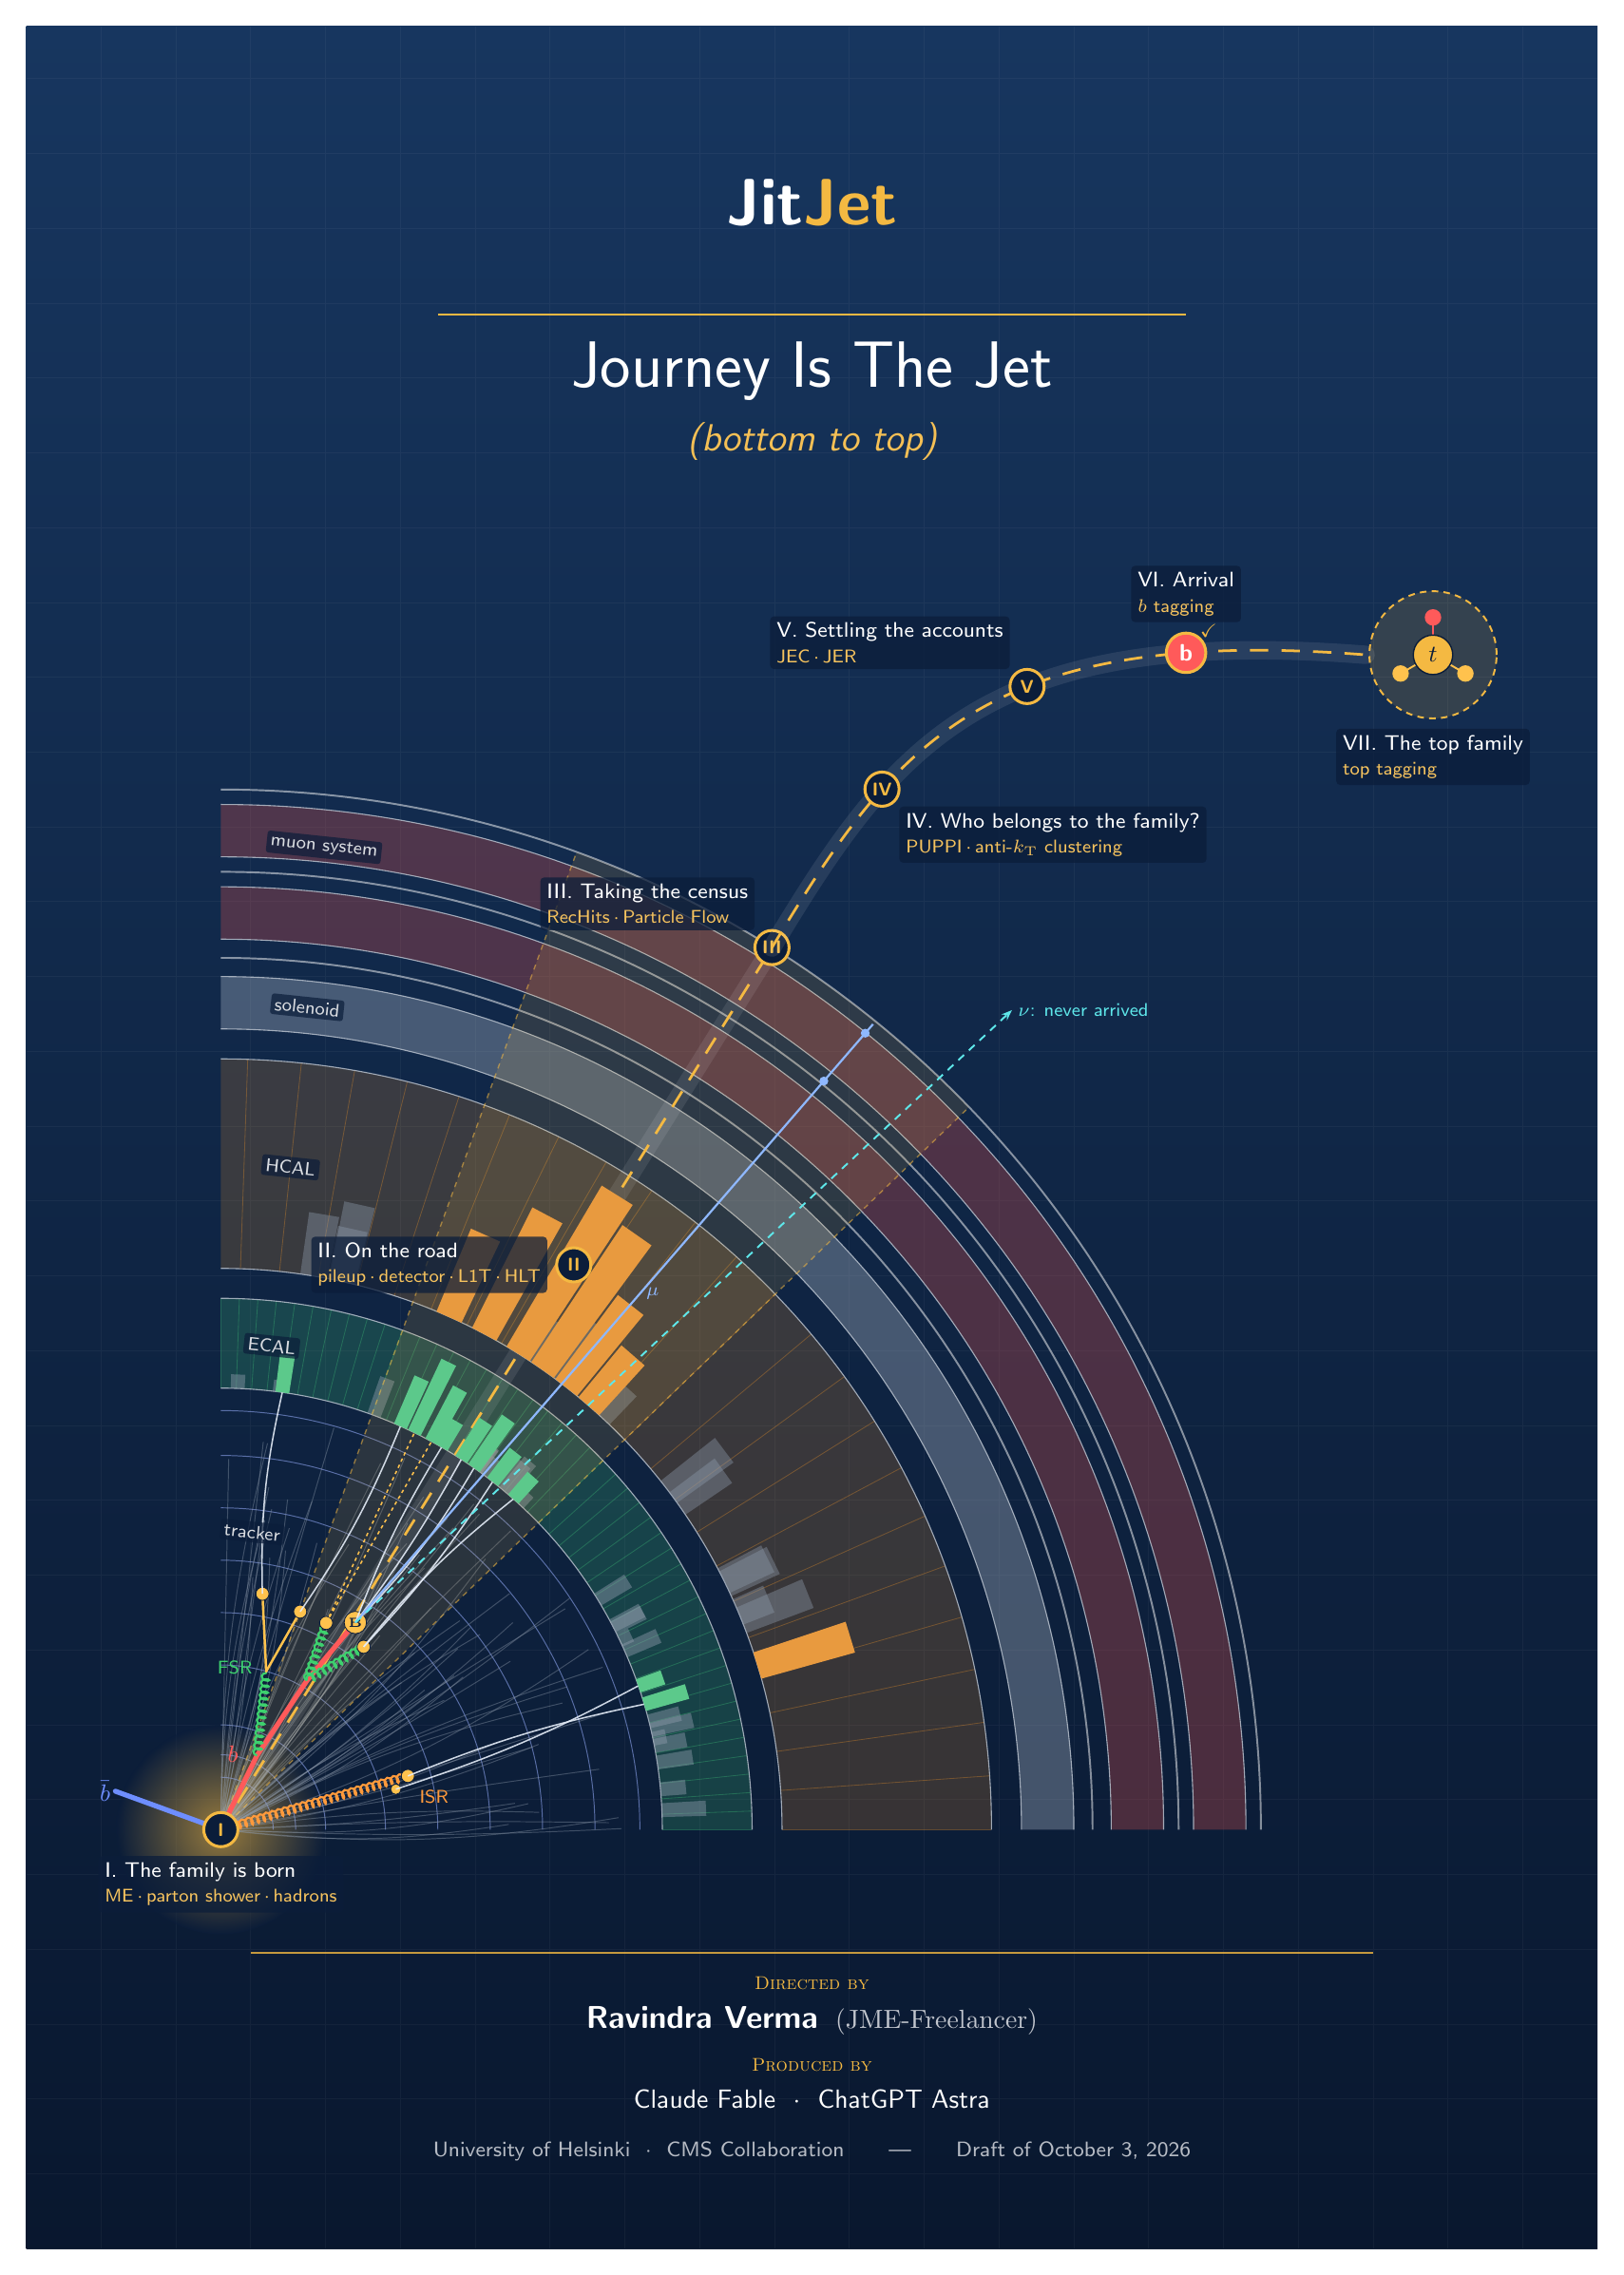
\begin{tikzpicture}[x=1cm,y=1cm]
\useasboundingbox (0,0) rectangle (21,29.7);
\clip (0,0) rectangle (21,29.7);

%% ======== background ========================================================
\shade[top color=navytop, bottom color=navy!80!black] (0,0) rectangle (21,29.7);
\draw[white, opacity=0.045, line width=0.3pt, step=1cm] (0,0) grid (21,29.7);

\coordinate (IP) at (2.6,5.6);

%% ======== the detector: a transverse quarter of CMS =========================
\begin{scope}[shift={(IP)}]
  % the glow of the hard scattering
  \shade[inner color=gold, outer color=navy, opacity=0.6] (0,0) circle[radius=1.4];

  % tracker: pixel and strip layers
  \foreach \r in {0.7,1.0,1.4,2.2,2.9,3.6,4.3,5.0,5.6}
    \draw[tracklayer] (0:\r) arc[start angle=0, end angle=90, radius=\r];
  % ECAL crystals
  \fill[ecalcol, opacity=0.22] (0:5.9) arc[start angle=0, end angle=90, radius=5.9]
    -- (90:7.1) arc[start angle=90, end angle=0, radius=7.1] -- cycle;
  \foreach \a in {0,2,...,90} \draw[ecalcol, opacity=0.35, line width=0.3pt] (\a:5.9) -- (\a:7.1);
  \draw[ring] (0:5.9) arc[start angle=0, end angle=90, radius=5.9];
  \draw[ring] (0:7.1) arc[start angle=0, end angle=90, radius=7.1];
  % HCAL towers
  \fill[hcalcol, opacity=0.20] (0:7.5) arc[start angle=0, end angle=90, radius=7.5]
    -- (90:10.3) arc[start angle=90, end angle=0, radius=10.3] -- cycle;
  \foreach \a in {0,4,...,90} \draw[hcalcol, opacity=0.35, line width=0.3pt] (\a:7.5) -- (\a:10.3);
  \draw[ring] (0:7.5) arc[start angle=0, end angle=90, radius=7.5];
  \draw[ring] (0:10.3) arc[start angle=0, end angle=90, radius=10.3];
  % solenoid
  \fill[steel, opacity=0.40] (0:10.7) arc[start angle=0, end angle=90, radius=10.7]
    -- (90:11.4) arc[start angle=90, end angle=0, radius=11.4] -- cycle;
  \draw[ring] (0:10.7) arc[start angle=0, end angle=90, radius=10.7];
  \draw[ring] (0:11.4) arc[start angle=0, end angle=90, radius=11.4];
  % muon system: return yoke (red) with muon chambers (white arcs) between
  \foreach \ri/\ro in {11.9/12.6, 13.0/13.7}{
    \fill[yoke, opacity=0.35] (0:\ri) arc[start angle=0, end angle=90, radius=\ri]
      -- (90:\ro) arc[start angle=90, end angle=0, radius=\ro] -- cycle;
    \draw[ring] (0:\ri) arc[start angle=0, end angle=90, radius=\ri];
    \draw[ring] (0:\ro) arc[start angle=0, end angle=90, radius=\ro];}
  \foreach \r in {11.65,12.8,13.9}
    \draw[white, opacity=0.5, line width=0.7pt] (0:\r) arc[start angle=0, end angle=90, radius=\r];

  % pileup: the crowd on the road, tracks from the same interaction point
  \pgfmathsetseed{2026}
  \foreach \i in {1,...,70}{
    \pgfmathsetmacro{\a}{90*rnd}
    \pgfmathsetmacro{\b}{9*rand}
    \pgfmathsetmacro{\r}{5.6*(0.55+0.45*rnd)}
    \draw[putrack] (0,0) to[bend left=\b] (\a:\r);}
  \foreach \i in {1,...,22}{
    \pgfmathsetmacro{\a}{2+86*rnd}
    \pgfmathsetmacro{\h}{0.15+0.45*rnd}
    \ecalbar{\a}{\h}{pu, opacity=0.45}}
  \foreach \i in {1,...,12}{
    \pgfmathsetmacro{\a}{3+84*rnd}
    \pgfmathsetmacro{\h}{0.2+0.9*rnd}
    \hcalbar{\a}{\h}{pu, opacity=0.40}}

  % the jet cone (anti-kT R): everything inside is "the jet"
  \fill[gold, opacity=0.13] (0,0) -- (44:13.9) arc[start angle=44, end angle=70, radius=13.9] -- cycle;
  \draw[gold, opacity=0.55, dash pattern=on 2pt off 2pt, line width=0.5pt] (0,0) -- (44:13.9) (0,0) -- (70:13.9);

  % the road: the jet axis
  \draw[road] (0,0) -- (58:13.9);
  \draw[roadline] (0,0) -- (58:13.9);
  \coordinate (E) at (58:13.9);

  % the mother quark and her children: parton shower
  \coordinate (P1) at (64:1.1);
  \coordinate (P2) at (60:2.3);
  \coordinate (P3) at (57:3.3);
  \coordinate (G1) at (74:2.2);
  \coordinate (G2) at (63:3.1);
  \coordinate (G3) at (52:3.1);
  \coordinate (Q1) at (80:3.2);
  \coordinate (Q2) at (70:3.1);
  \coordinate (I1) at (16:2.6);
  \draw[bbarline] (0,0) -- (160:1.5) node[left, bblue, font=\small\bfseries, inner sep=1pt] {$\bar b$};
  \draw[isrgluon] (0,0) -- (I1);
  \draw[bline] (0,0) -- (P1) -- (P2) -- (P3);
  \draw[gluon] (P1) -- (G1);
  \draw[gluon] (P2) -- (G2);
  \draw[gluon] (P2) -- (G3);
  \draw[quark] (G1) -- (Q1);
  \draw[quark] (G1) -- (Q2);
  \node[bred, font=\small\bfseries, inner sep=1pt] at ($(P1)+(-0.32,0.02)$) {$b$};
  \node[isr, font=\scriptsize\sffamily, inner sep=1pt] at ($(I1)+(0.35,-0.28)$) {ISR};
  \node[fsr, font=\scriptsize\sffamily, inner sep=1pt] at ($(G1)+(-0.42,0.05)$) {FSR};

  % hadronisation: the children get dressed
  \foreach \p in {G2,G3,Q1,Q2,I1} \node[hadron] at (\p) {};
  \node[hadron, minimum size=8.5pt, font=\tiny\bfseries, text=navy] at (P3) {B};
  \node[hadron, minimum size=4pt] at (13:2.4) {};

  % tracks in the magnetic field, to the ECAL surface
  \draw[track] (Q1) to[bend left=7] (82:5.9);
  \draw[track] (Q2) to[bend right=6] (66:5.9);
  \draw[photon] (G2) -- (64:5.9);
  \draw[photon] (G2) -- (61.5:5.9);
  \draw[track] (G3) to[bend left=6] (48.5:5.9);
  \draw[track] (G3) to[bend right=5] (52:5.9);
  \draw[track] (P3) to[bend left=5] (60:5.9);
  \draw[track] (P3) to[bend right=4] (57:5.9);
  \draw[track] (P3) to[bend right=7] (55:5.9);
  \draw[track] (I1) to[bend left=5] (16.5:5.9);
  \draw[track] (13:2.4) to[bend right=5] (19:5.9);

  % calorimeter deposits of the jet
  \foreach \a/\h in {82/0.5, 66/0.7, 64/1.05, 61.5/0.8, 60/0.4, 57/0.6, 55/0.8, 52/0.5, 48.5/0.4, 16.5/0.6, 19/0.35}
    {\ecalbar{\a}{\h}{ecalcol!85!white}}
  \foreach \a/\h in {66/1.2, 62/1.8, 58/2.5, 55/2.2, 52/1.4, 49/0.9, 17/1.3}
    {\hcalbar{\a}{\h}{hcalcol!90!white}}

  % the muon from the B decay reaches the muon chambers ...
  \draw[draw=muoncol, line width=0.8pt] (P3) -- (51:13.85)
    node[pos=0.905, circle, fill=muoncol, inner sep=1.2pt] {}
    node[pos=0.985, circle, fill=muoncol, inner sep=1.2pt] {}
    node[pos=0.55, right=1pt, muoncol, font=\scriptsize\sffamily, inner sep=1pt] {$\mu$};
  % ... and the neutrino never arrives
  \draw[draw=nucol, line width=0.7pt, dash pattern=on 3pt off 2.5pt, -{Stealth[length=4pt]}]
    (P3) -- ($(P3)+(43:12)$) node[right, nucol, font=\scriptsize\sffamily, inner sep=2pt] {$\nu$: never arrived};

  % names of the layers
  \node[layerlabel, rotate=-6] at (84:4.0) {tracker};
  \node[layerlabel, rotate=-6] at (84:6.5) {ECAL};
  \node[layerlabel, rotate=-6] at (84:8.9) {HCAL};
  \node[layerlabel, rotate=-6] at (84:11.05) {solenoid};
  \node[layerlabel, rotate=-6] at (84:13.2) {muon system};

  % milestones inside the detector
  \node[milestone] (m1) at (0,0) {I};
  \node[mlabel, anchor=north] at ($(m1.south)+(0,-0.1)$) {I. The family is born\sub{ME\,$\cdot$\,parton shower\,$\cdot$\,hadrons}};
  \node[milestone] (m2) at (58:8.9) {II};
  \node[mlabel, anchor=east] at ($(m2.west)+(-0.1,0)$) {II. On the road\sub{pileup\,$\cdot$\,detector\,$\cdot$\,L1T\,$\cdot$\,HLT}};
  \node[milestone] (m3) at (E) {III};
  \node[mlabel, anchor=south east] at ($(m3.north west)+(-0.05,0.05)$) {III. Taking the census\sub{RecHits\,$\cdot$\,Particle Flow}};
\end{scope}

%% ======== the road beyond the detector: reconstruction to the top ===========
\draw[road] (E) .. controls (11.6,20.1) and (12.8,21.7) .. (17.9,21.3);
\draw[roadline] (E) .. controls (11.6,20.1) and (12.8,21.7) .. (17.9,21.3)
  coordinate[pos=0.30] (m4c) coordinate[pos=0.60] (m5c) coordinate[pos=0.82] (m6c);

\node[milestone] (m4) at (m4c) {IV};
\node[mlabel, anchor=north west] at ($(m4.south east)+(0.05,-0.05)$) {IV. Who belongs to the family?\sub{PUPPI\,$\cdot$\,anti-$k_{\mathrm{T}}$ clustering}};
\node[milestone] (m5) at (m5c) {V};
\node[mlabel, anchor=south east] at ($(m5.north west)+(-0.05,0.05)$) {V. Settling the accounts\sub{JEC\,$\cdot$\,JER}};
% VI: the registry office stamps the b-jet
\node[circle, draw=gold, fill=bred, line width=1.1pt, minimum size=15pt, inner sep=0pt,
      font=\sffamily\bfseries\small, text=white] (m6) at (m6c) {b};
\node[gold, font=\scriptsize\bfseries] at ($(m6)+(0.30,0.30)$) {\checkmark};
\node[mlabel, anchor=south] at ($(m6.north)+(0,0.12)$) {VI. Arrival\sub{$b$ tagging}};
% VII: the top family, a three-prong fat jet
\coordinate (T) at (18.8,21.3);
\draw[gold, dash pattern=on 2.5pt off 2pt, line width=0.7pt] (T) circle[radius=0.85];
\fill[gold, opacity=0.15] (T) circle[radius=0.85];
\foreach \a/\c in {90/bred, 210/hadroncol, 330/hadroncol}{
  \draw[draw=\c, line width=0.7pt] (T) -- ($(T)+(\a:0.5)$);
  \fill[\c] ($(T)+(\a:0.5)$) circle[radius=0.11];}
\node[circle, fill=gold, draw=navy, line width=0.5pt, minimum size=15pt, inner sep=0pt,
      font=\sffamily\bfseries\small, text=navy] at (T) {$t$};
\node[mlabel, anchor=north] at ($(T)+(0,-0.98)$) {VII. The top family\sub{top tagging}};

%% ======== title =============================================================
\node[anchor=center] at (10.5,27.35)
  {\fontsize{84}{88}\selectfont\sffamily\bfseries{\color{white}Jit}{\color{gold}Jet}};
\draw[gold, line width=0.8pt] (5.5,25.85) -- (15.5,25.85);
\node[anchor=center, white, font=\fontsize{27}{30}\selectfont\sffamily] at (10.5,25.1) {Journey Is The Jet};
\node[anchor=center, gold!90!white, font=\fontsize{15}{18}\selectfont\sffamily\itshape] at (10.5,24.15) {(bottom to top)};

%% ======== credits ===========================================================
\draw[gold, line width=0.6pt, opacity=0.8] (3,3.95) -- (18,3.95);
\node[anchor=center, gold, font=\sffamily\scriptsize\scshape] at (10.5,3.55) {Directed by};
\node[anchor=center, white, font=\sffamily\bfseries\large] at (10.5,3.05)
  {Ravindra Verma \,{\normalfont\normalsize\color{white!75!navy}(JME-Freelancer)}};
\node[anchor=center, gold, font=\sffamily\scriptsize\scshape] at (10.5,2.45) {Produced by};
\node[anchor=center, white, font=\sffamily\normalsize] at (10.5,2.0) {Claude Fable\ \ $\cdot$\ \ ChatGPT Astra};
\node[anchor=center, white!70!navy, font=\sffamily\footnotesize] at (10.5,1.3)
  {University of Helsinki\ \ $\cdot$\ \ CMS Collaboration\qquad|\qquad Draft of \today};

\end{tikzpicture}
\end{document}
